
\section{Results}\notinsubfile{\label{sec:results}}
%\setcounter{page}{0}\pagenumbering{arabic}

\subsubsection{The model with no returns heterogeneity}

\par To solve and simulate the model, I follow the calibration scheme captured in table \ref{tab:calib1}.
\hypertarget{calibPY}{}
\begin{table}[ht]
  \centering
  \resizebox{0.7\textwidth}{!}{
    \begin{tabular}{cccc}
        \toprule
        Description & Parameter & Value & Source \\
        \midrule
        Time discount factor & $\beta$ & 0.99 & \cite{Den_Haan2010} \\
        CRRA & $\rho$ & 1 & \cite{Den_Haan2010} \\
        Capital share & $\alpha$ & 0.36 & \cite{Den_Haan2010} \\
        Depreciation rate & $\delta$ & 0.025 & \cite{Den_Haan2010} \\
        Time worked per employee & $\ell$ & 1/.09 & \cite{Den_Haan2010} \\
        Capital/output ratio & $\frac{K}{Y}$ & 10.26 & \cite{Den_Haan2010} \\
        Effective interest rate & $r - \delta$ & 0.01 & \cite{Den_Haan2010} \\
        Wage rate & $W$ & 2.37 & \cite{Den_Haan2010} \\
        Unempl. insurance payment & $\mu$ & 0.15 & \cite{Den_Haan2010} \\
        Probability of death & $D$ & 0.00625 & Yields 40-year working life \\
        Variance of $\log \theta_{t,i}$ & $\sigma^{2}_{\theta}$ & 0.010 x 4 & \begin{tabular}[t]{@{}p{5.5cm}@{}} \cite{Carroll1992}, \\ \cite{Carroll2015} \end{tabular} \\
        Variance of $\log \psi_{t,i}$ & $\sigma^{2}_{\psi}$ & 0.010 x 4/11 & \begin{tabular}[t]{@{}p{5.5cm}@{}} \cite{Carroll1992}, \\  \cite{Debacker2013},  \\ \cite{Carroll2015} \end{tabular} \\
        Unemployment rate & $\mho$ & 0.07 & Mean in \cite{Den_Haan2010} \\
        \bottomrule
    \end{tabular}
    }
    \caption{Parameter values (quarterly frequency) for the perpetual youth (infinite horizon) model.}
    \label{tab:calib1}
\end{table}

\unskip

\par The solution of the model with no heterogeneity in returns (the R-point model) is the one which finds the value for the rate of return $R$ which minimizes the distance between the simulated and empirical wealth shares at the 20th, 40th, 60th, and 80th percentiles. The empirical targets are computed using the 2004 SCF data on household wealth. The estimation procedure finds this optimal value to be $R = 1.0602$.

\subsubsection{Incorporating heterogeneous returns}

\par As noted above, recent studies by \cite{aflgdmlp20} and \cite{lblcps18} have not only estimated the rate of return on asset holdings but have also uncovered significant heterogeneity across households. With this in mind, the next estimation (the R-dist model) assumes the existence of multiple types of agents, each earning a distinct rate of return on their assets.

\par I follow closely the procedure outlined by \cite{cstw2017}. Specifically, I assume that different types of households have a time preference factor drawn from a uniform distribution on the interval $(\grave{R} - \nabla, \grave{R} + \nabla)$, where $\nabla$ represents the level of dispersion. Afterward, the model is simulated to estimate the values of both $\grave{R}$ and $\nabla$ so that the model matches the inequality in the wealth distribution. To achieve this, the following minimization problem is solved:

$$ \{\grave{R}, \nabla\} = \text{arg}\min_{R, \nabla} \bigg( \sum_{i=20, 40, 60, 80} (w_{i}(R, \nabla)-\omega_i )^{2} \bigg)^{\frac{1}{2}} $$

\par subject to the constraint that the aggregate capital-to-output ratio in this model matches the calibrated value $5$. This is towards the upper bound on plausibly calibrated values for the capital-to-output ratio, as much of the literature chooses values between $2$ and  $3$.

\par Note that $w_i$ and $\omega_i$ give the porportion of total aggregate net worth held by the top $i$ percent in the model and in the data, respectively.

\par The estimation procedure finds this optimal values of $R = 1.0212$ and $\nabla = 0.06728$. These parameter values pin down the estimated uniform distribution. In the model, I've chosen to discretize that distribution to 7 chosen points. The performance of the estimation of both the R-point and R-dist models, measured by their ability to match the SCF data, is compared in figure \ref{fig:PYUnif}.

\begin{figure}[h]
    \centering
    \begin{minipage}{0.48\textwidth}
        \centering
        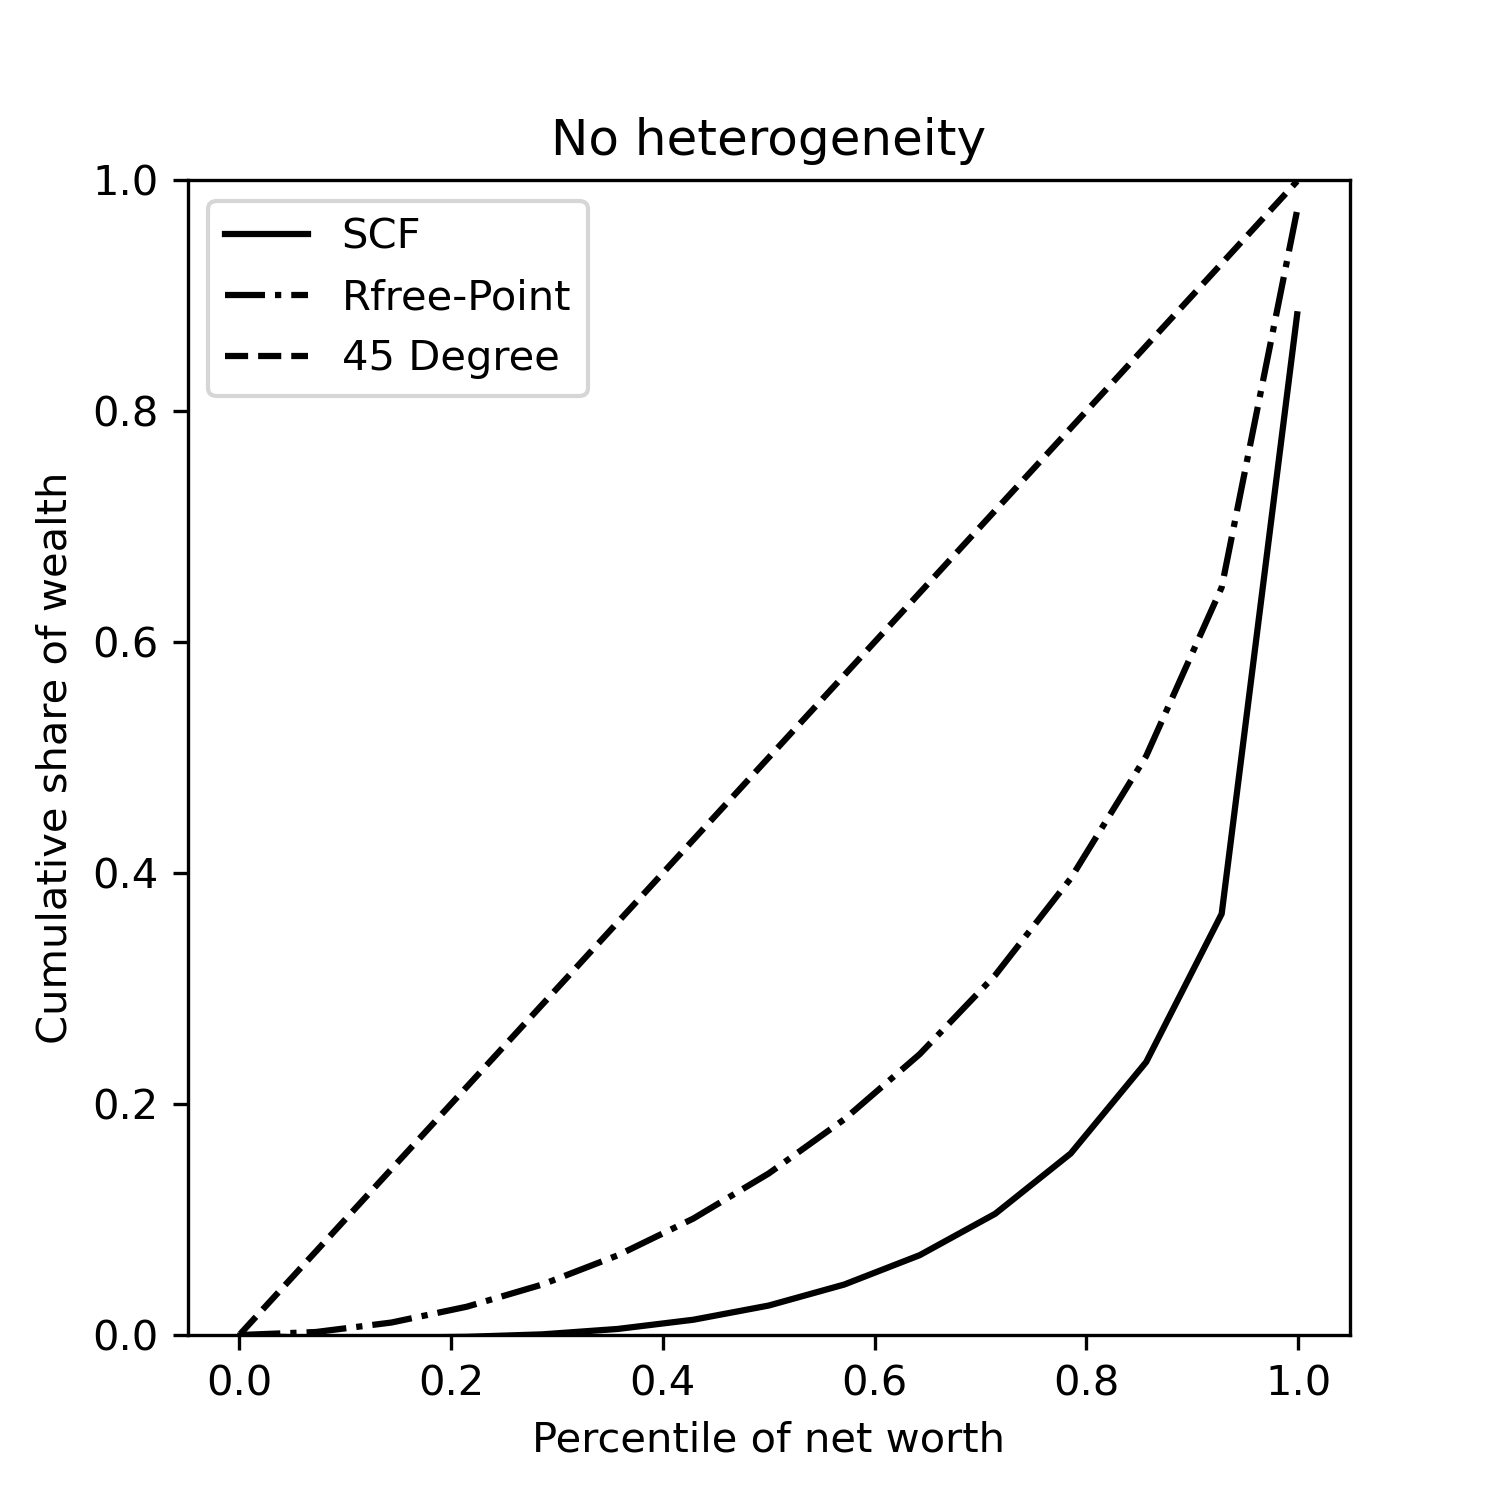
\includegraphics[width=\textwidth]{../Figures/PYrrPointNetWorthPlot.png}
    \end{minipage}
    \hfill
    \begin{minipage}{0.48\textwidth}
        \centering
        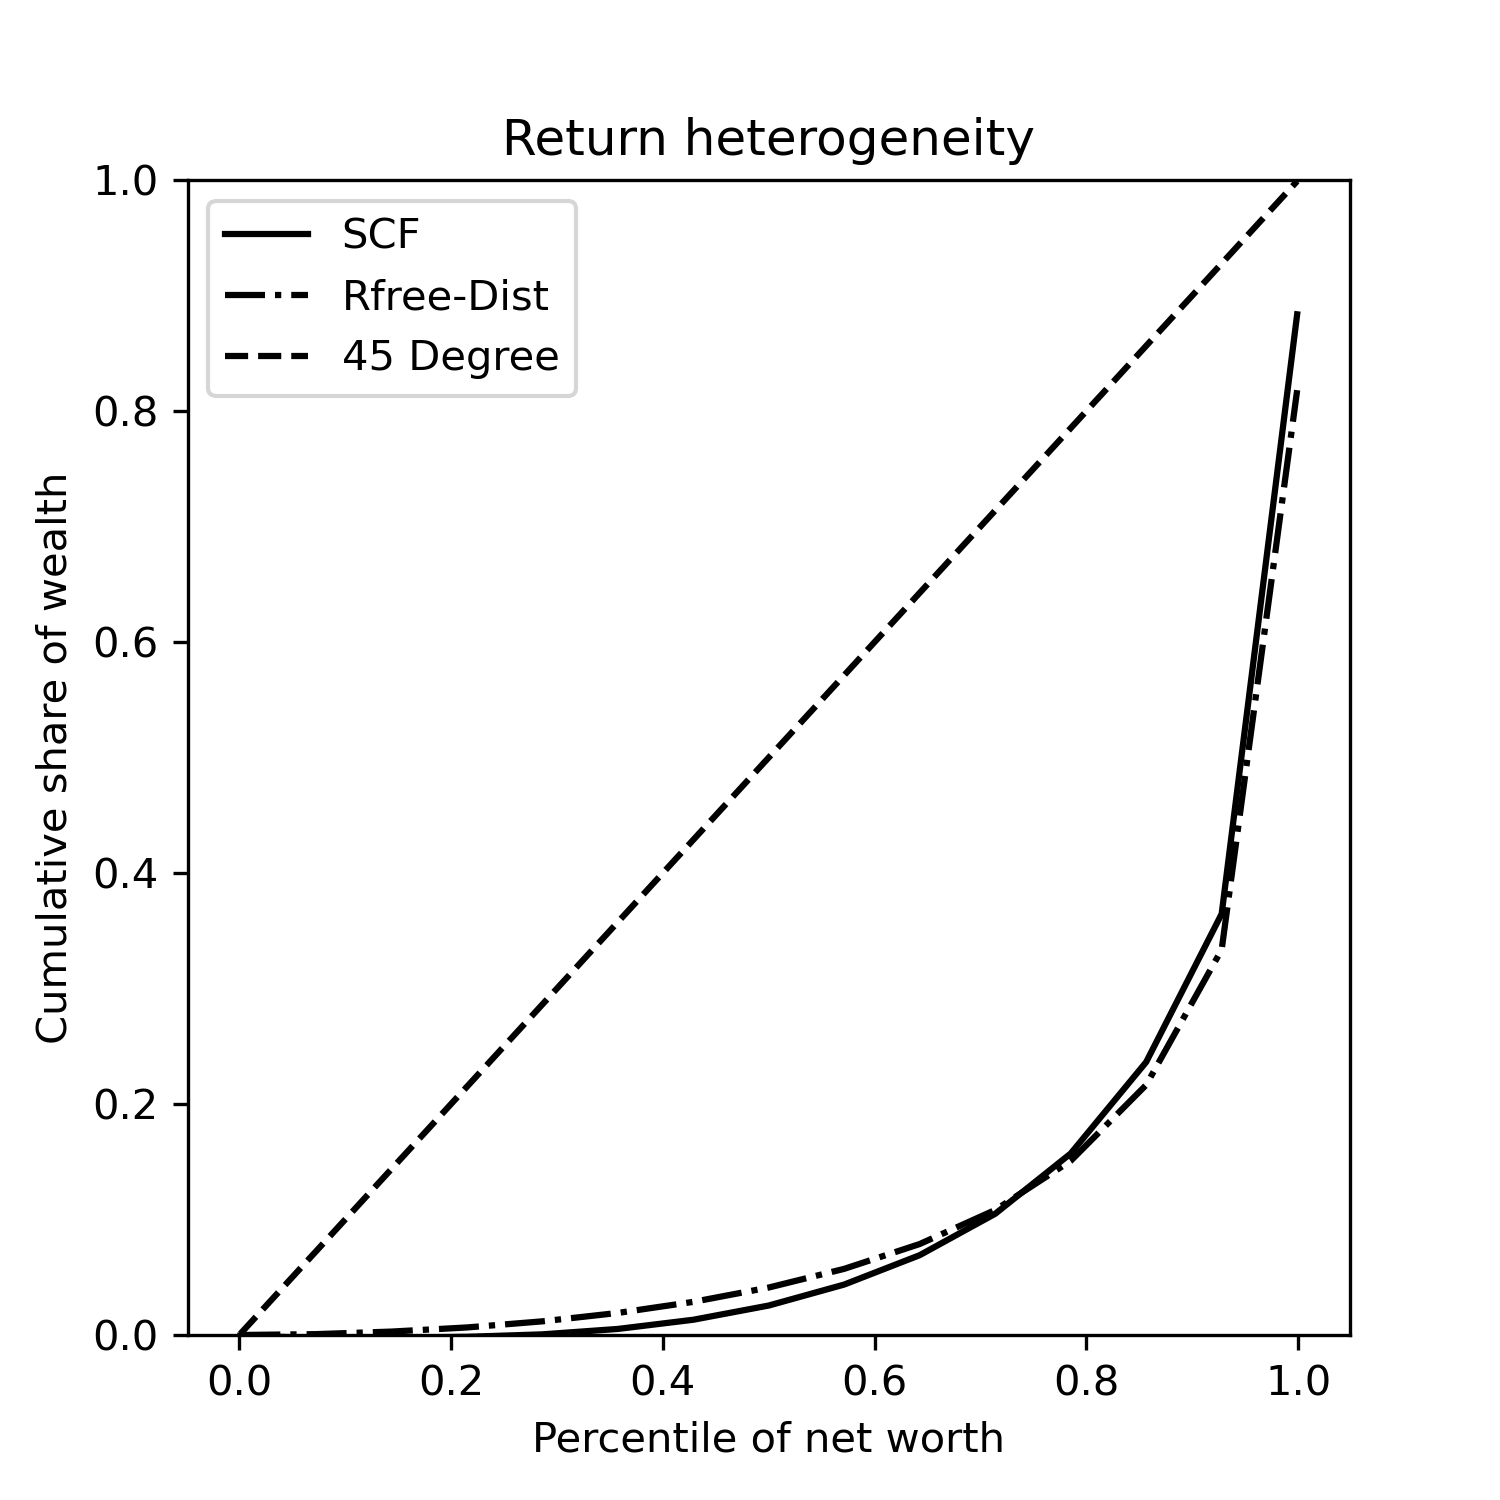
\includegraphics[width=\textwidth]{../Figures/PYrrDistNetWorthPlot.png}
    \end{minipage}
    \caption{Comparison of R-Point and R-Dist Models.}
    \label{fig:PYUnif} 
\end{figure}

 \subsubsection{The implied distribution of bank heterogeneity}

  \par I've estimated the distribution of returns which matches the wealth moments. As mentioned earlier, I can use this and the assumptions regarding the bank's decision problem to back out an implied distribution of $\varepsilon$. This will describe how the banks differ in the sensitivity of their deposit levels to changes in the market interest rate. Both in our simplified setting, and in the transmission channel empirically documented by \cite{Drechsler2017}, differences in these sensitivities ultimately leads to differences in the deposit rates offered across banks.  

  \par First, I assume that the aggregate production function is Cobb-douglas, so that the marginal product of capital can be written as $\alpha \frac{Y}{K}$. With the calibrated values  $\delta = .025$, $\alpha = .36$, and the capital to output ratio $3$, this setting has an effective interest rate of $R^m = 1.095$ which can be used as the market interest rate.

  \par Since the model with heterogeneity (i.e. the R-dist model) has 7 estimated points for the uniform distribution, the implied, estimated points for $\varepsilon$ can be uniquely pineed down by the expression $$\varepsilon_i = \frac{R_i^d}{R^m - R_i^d} .$$

  \par For the infinte horizon version of the model which matches 2004 SCF data on net worth, the 7 estimated points describing heterogeneous returns are \texttt{[0.9635, 0.9828, 1.0012, 1.0212, 1.0404, 1.0596, 1.0789]}. The corresponding 7 implied elasticities are given by \texttt{[7.3288, 8.7552, 10.7712, 13.8374, 19.0636, 29.9737, 66.8914]}.

 
\subsection{Incorporating life cycle dynamics into the model}

\par More realistic assumptions regarding the age and education level of households can have important implications for the income and mortality process of households. Here, I extend the model to incorporate these life cycle dynamics.

\par Households enter the economy at time $t$ aged 24 years old and are endowed with an education level $e \in \{D,HS,C\}$, and initial permanent income level $\textbf{p}_0$, and a capital stock $k_0$. The life cycle version of household income is given by:

$$ y_t = \xi_t \textbf{p}_t = (1 - \tau) \theta_t \textbf{p}_t, $$

where $\textbf{p}_t = \psi_t \bar{\psi}_{es} \textbf{p}_{t-1}$ and $\bar{\psi}_{es}$ captures the age-education-specific average growth factor. Households that have lived for $s$ periods have permanent shocks drawn from a lognormal distribution with mean $1$ and variance $\sigma^{2}_{\psi s}$ and transitory shocks drawn from a lognormal distribution with mean $\frac{1}{\cancel{\mho}}$ and variance $\sigma^{2}_{\theta s}$ with probability $\cancel{\mho} = (1-\mho)$ and $\mu$ with probability $\mho$.

\par The normalized version of the age-education-specific consumption-saving problem for households is given by

\begin{eqnarray*}
  v_{es}(m_t) &=& \max_{c_t} u(c_t(m_t)) + \beta \cancel{D}_{es} \mathbb{E}_{t}[\psi_{t+1}^{1-\rho}v_{es + 1}(m_{t+1})] \\
  &\text{s.t.}& \\
  a_t &=& m_t - c_t, \\
  k_{t+1} &=& \frac{a_t}{\psi_{t+1}}, \\
  m_{t+1} &=& (\daleth + r_t)k_{t+1} + \xi_{t+1}, \\
  a_t &\geq& 0.
\end{eqnarray*}

\par The additional parameters necessary to calibrate the life cycle version of the model are given in table \ref{tab:calib2}. The age-education dependent mean income levels come from \cite{Cagetti2003}. The permanent and transitory shock variances come from \cite{Sabelhaus2010}. The age-education dependent mortality rates come from \cite{Brown2007}.

\hypertarget{calibLC}{}
\begin{table}[ht]
  \centering
  \resizebox{0.6\textwidth}{!}{
    \begin{tabular}{ccc}
        \toprule
        Description & Parameter & Value  \\
        \midrule
        Population growth rate & $N$ & 0.0025  \\
        Technological growth rate & $\Gamma$ & 0.0037  \\
        Rate of high school dropouts & $\theta_D $ & 0.11  \\
        Rate of high school graduates & $\theta_{HS} $ & 0.55  \\
        Rate of college graduates & $\theta_C $ & 0.34  \\
        Labor income tax rate & $\tau$ & 0.0942  \\
        \bottomrule
    \end{tabular}}
    \caption{Parameter values (annual frequency) for the lifecycle model.}
    \label{tab:calib2}
\end{table}

\unskip

\par The estimation procedure finds this optimal value to be $R = 1.0414$ for the R-point model in this setting. The estimation procedure for the R-dist model in the life cycle setting finds optimal values of $R = 1.0343$ and $\nabla =0.03557$. Notice the improved performance of the estimation in matching the data displayed in figure \ref{fig:LCUnif}.

\begin{figure}[h]
    \centering
    \begin{minipage}{0.48\textwidth}
        \centering
        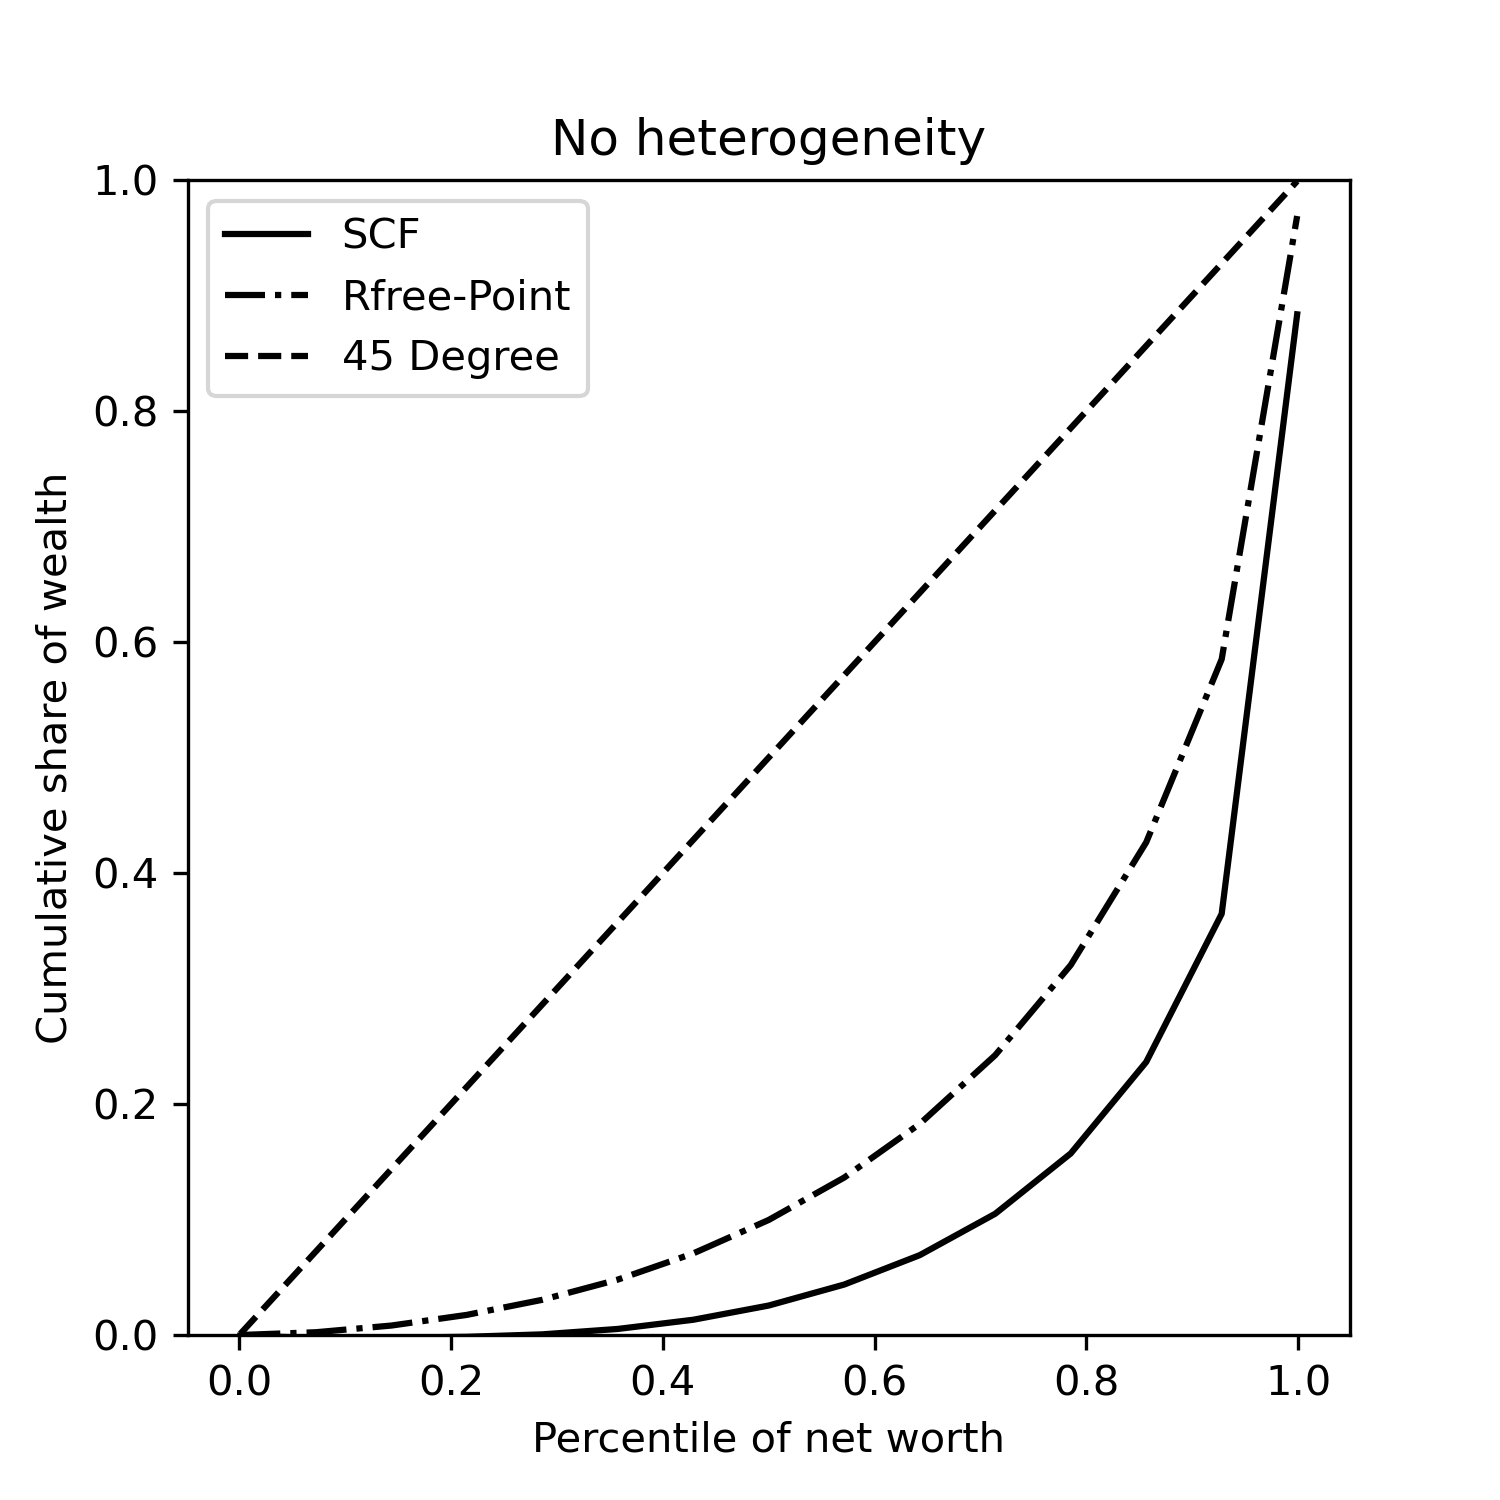
\includegraphics[width=\textwidth]{../Figures/LCrrPointNetWorthPlot.png}
    \end{minipage}
    \hfill
    \begin{minipage}{0.48\textwidth}
        \centering
        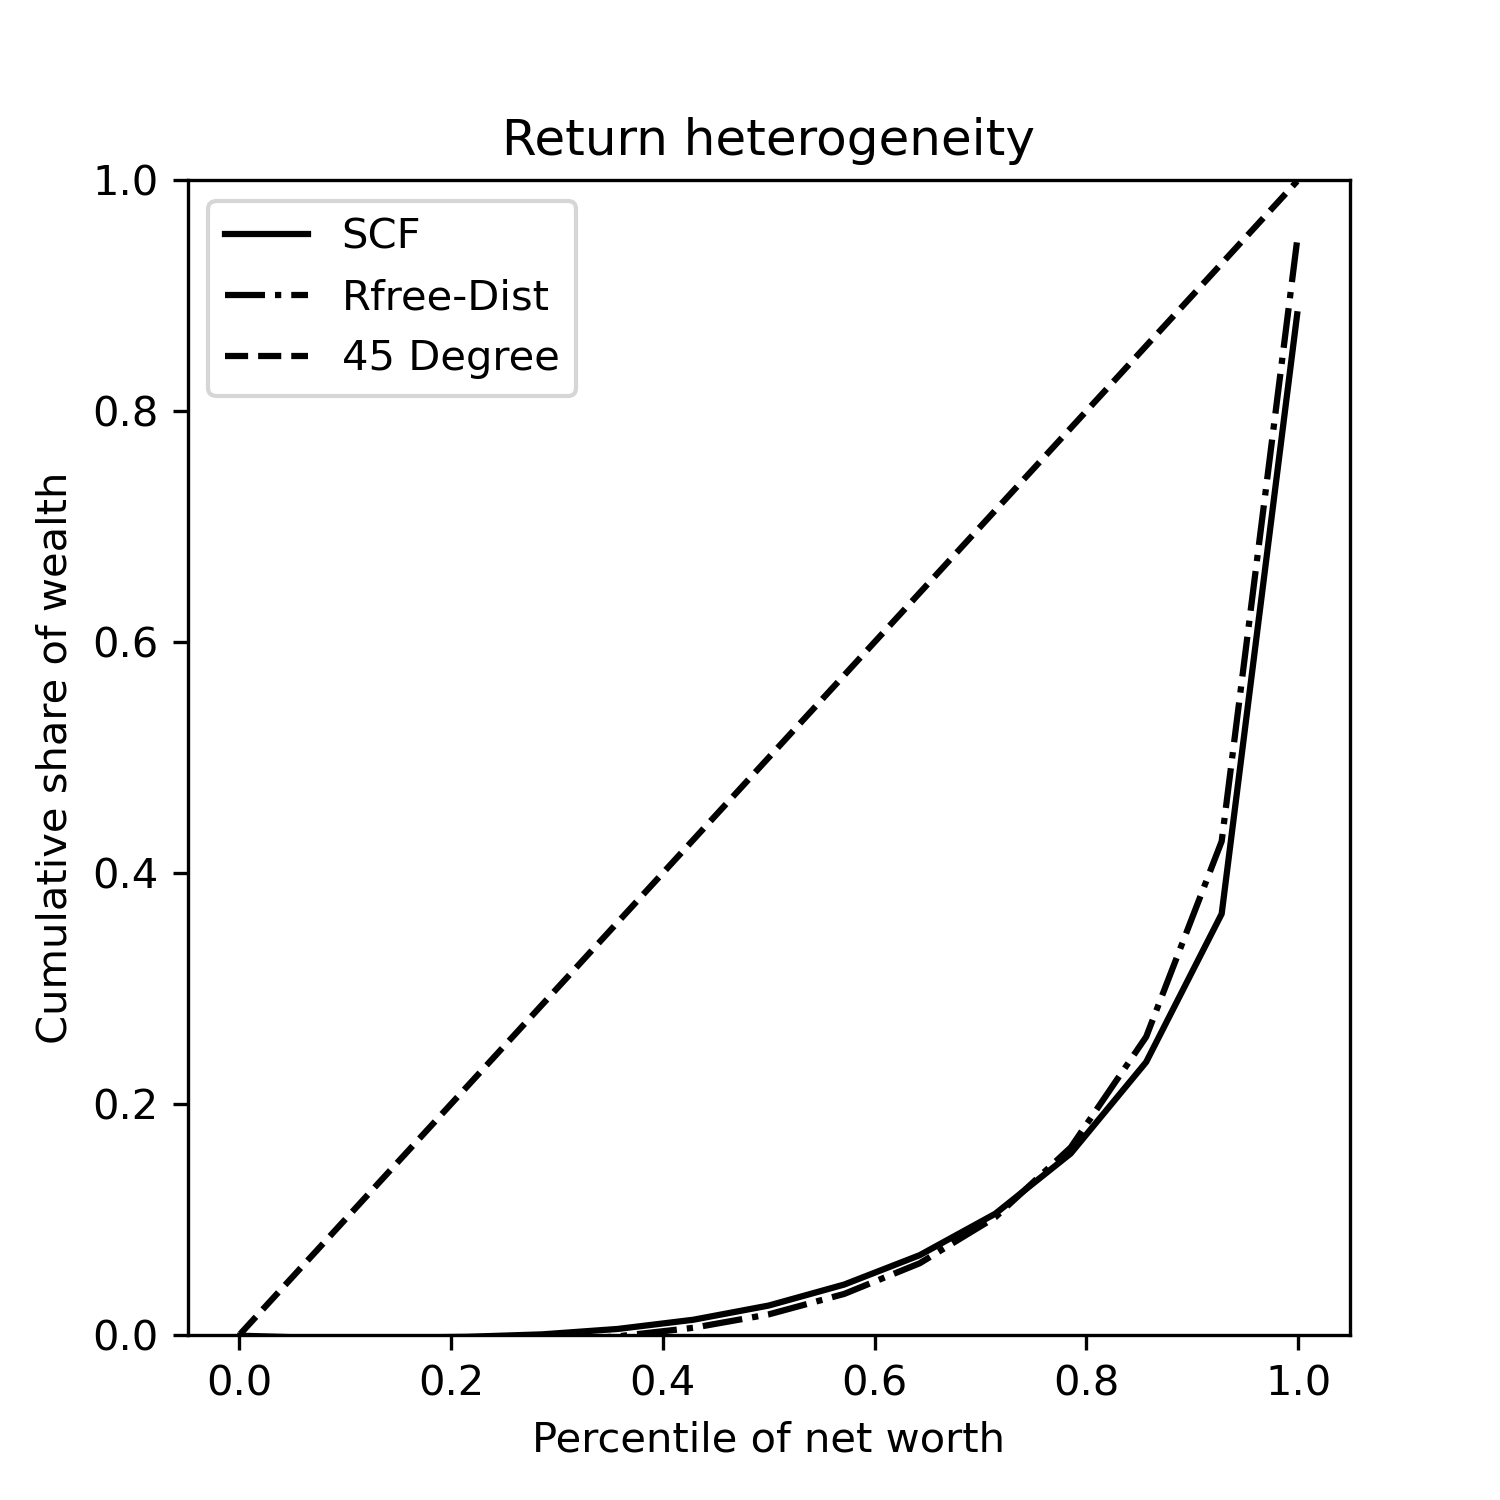
\includegraphics[width=\textwidth]{../Figures/LCrrDistNetWorthPlot.png}
    \end{minipage}
    \caption{Comparison of R-Point and R-Dist Models in the Life-Cycle Setting.}
    \label{fig:LCUnif} 
  \end{figure}

\par For the life cycle version of the model which matches 2004 SCF data on net worth, the 7 estimated points describing heterogeneous returns are \texttt{[0.9755, 0.9913, 1.0072, 1.0230, 1.0388, 1.0546, 1.0705]}. The corresponding 7 implied elasticities are given by \texttt{[8.1649, 9.5642, 11.4677, 14.2079, 18.4920, 26.1362, 43.6448]}.

\subsection{Assessing model performance}

\par The results presented thus far are encouraging for a number of reasons. First, these results are inline with a common finding in the heterogeneous agent literature, which is that a single source of ex-ante heterogeneity, even when there is only a single, riskless asset available to partially insure against uncertain labor income, is enough to drastically improve the models ability to generate a reasonably skewed wealth distribution. Second, I am also able to match moments similar to those in \cite{cstw2017}, which this model is a close analog of.

\par Although these are reasons to be encouraged by these results, they also suggest that assessing the model's performance only by how well it matches wealth moments is insufficient. To that end, I return to the literature on bank deposit sensitivities to changes in the federal funds rate. As we will see, the implied distribution of elasticities from my estimation method can be directly compared to those empirical estimatese, and how well they match can be used to assess my model. Additionally, I include wealth shares by age cohort as an additional set of untargeted moments for a similar assessment.  

\subsubsection{Interpreting the implied distribution of elasticities}

\par The usefulness in choosing a functional form for the level of deposits at a given bank as $S(\cdot) = A \left( \frac{R^d}{R^m} \right)^{\varepsilon}$ is that the parameter $\varepsilon$ has a clear interpretation as the elasticity of deposits to changes in the market interest rate. It can be shown that:

\[
-\varepsilon = \frac{\partial \ln S(\cdot)}{\partial \ln R^m}. 
\]

\par So, the elasticity parameter tells us how a percentage change in the market interest rate changes the level of deposit, in percent terms. This allows us to directly compare the implied elasticities following the SMM procedure to the emepirical evidence on the transmission channel described by \cite{Drechsler2017} regarding the relationship between the Fed funds rate and the level of deposits at banks. For example, \cite{Genay2004} finds that a $1\%$ change in the Fed funds rate leads to about a  $3\%$ to  $4\%$ change in the level of deposits, depending on the size of the bank.

\par The amount of returns heterogeneity required to match wealth inequality using only safe assets (i.e. bank deposits) will lead to vastly overstated elasticities for the resulting banking sector. This is not surprising. If bank wish to attract depositors in the face of an increasing Fed funds rate, they will need to offer a higher rate on deposits, regardless of the size of the bank. This suggests that there will be less variation in the optimal deposit rates offered across the banking sector. The banks which do not offer competitive deposit rates will likely find that their depositors switch to other safe investment technologies like money market funds. Since my model doesn't not match any moments regarding the number of banks in the economy, nor does it model returns heterogeneity by allowing for the choice between safe assets, it isn't too surprising that the elasticity of deposits to changes in the market interest rate is not well matched in this setting. That said, the ability of the model to back out a distribution of elasticities under the given assumptions is still useful. 

\subsubsection{Untargeted moments}

\par It is well-documented in the literature on heterogeneous agent modeling that, adding a source of (ex-ante) heterogeneous beyond the addition of labor income uncertainty to the representative agent framework will allow the simulated distribution of wealth to match moments of the empirical wealth distribution particularly well. So, although it is useful to see that the model with heterogeneous returns does a good job of matching the given lorenz targets, we need another way to assess the model's performance.

\par For this reason, I include age-dependent wealth moments from the same wave of the SCF to serve as untargeted moments~\ref{fig:EmpLorenzTar}. These can be found in the following table~\ref{fig:EmpLorenzTar}.

\begin{figure}[h]
\centering
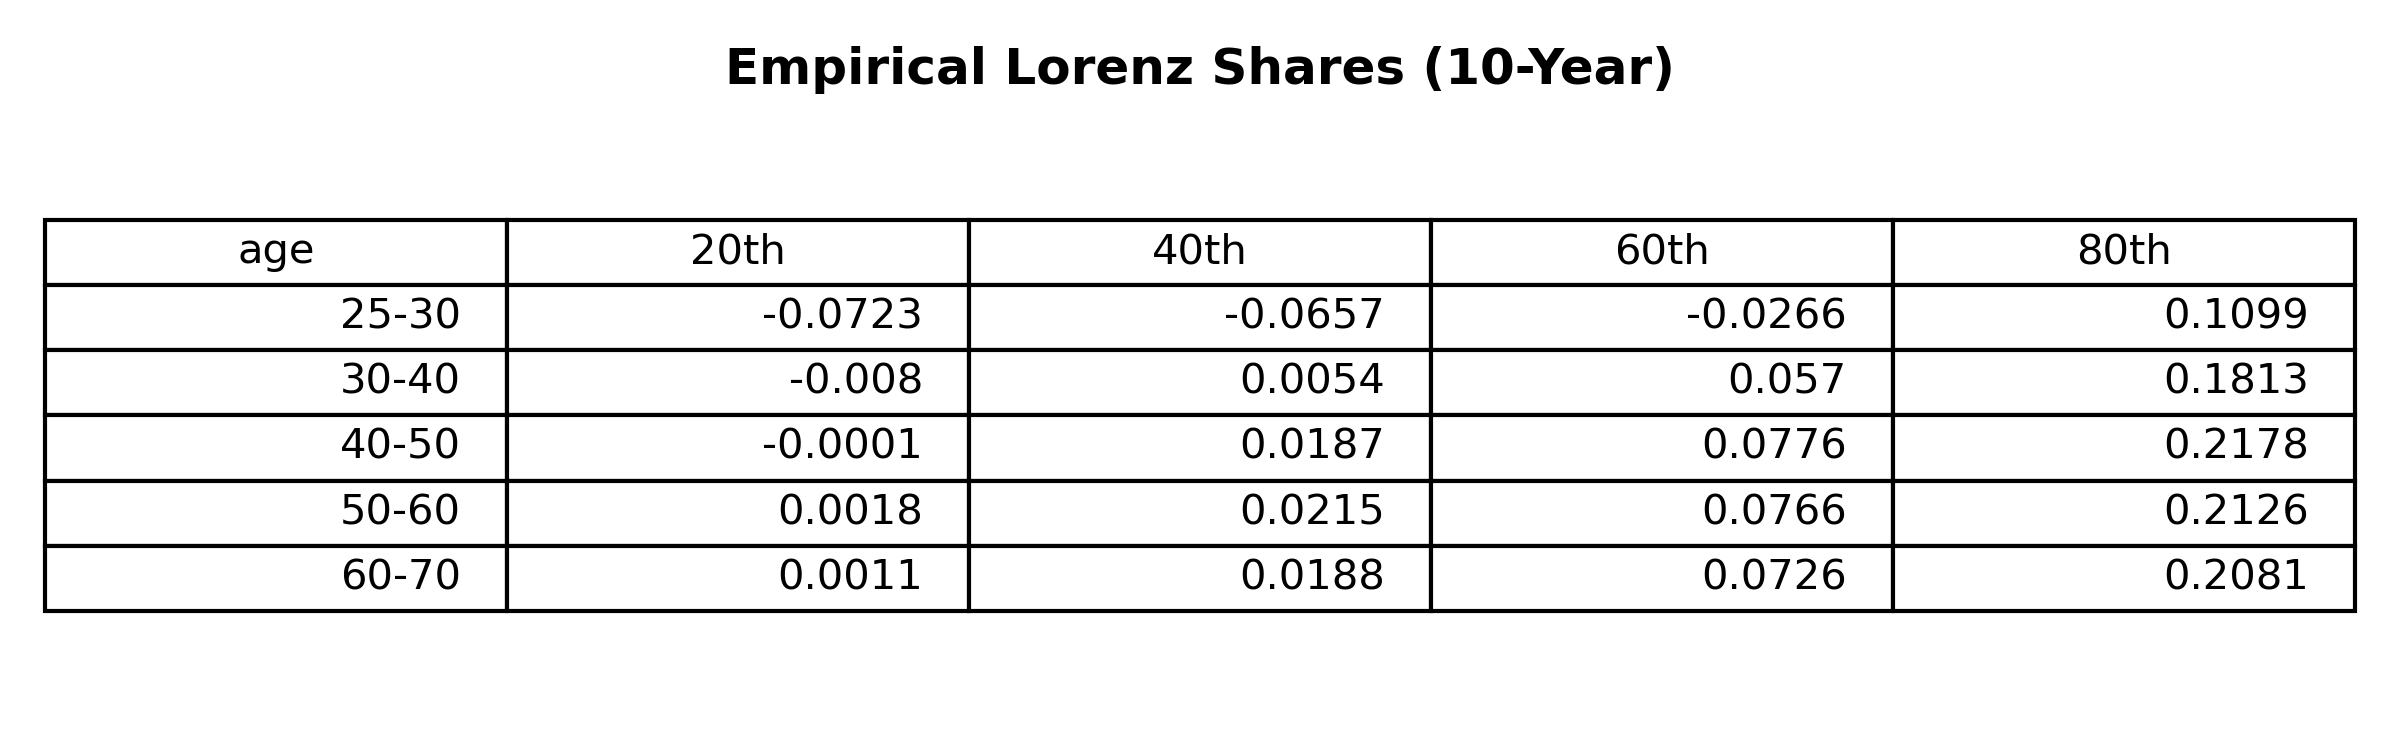
\includegraphics[width=0.8\textwidth]{Tables/Emp_Lorenz_10yr_LCrrDistNetWorth.png}
\caption{Empirical Lorenz Curve Targets from the 2004 SCF.}
\label{fig:EmpLorenzTar}
\end{figure}

\par The next two tables present the simulated version of the untargeted moments for the model without heterogeneity~\ref{fig:SimLorenzTarPoint}, and then with heterogeneity~\ref{fig:SimLorenzTarDist}. As you can see from the tables~\ref{fig:SimLorenzTarPoint} and~\ref{fig:SimLorenzTarDist} below, the age-dependent Lorenz targets that arise from the model again fit the data much better when returns heterogeneity is present versus when it is absent.

\begin{figure}[htbp]
\centering
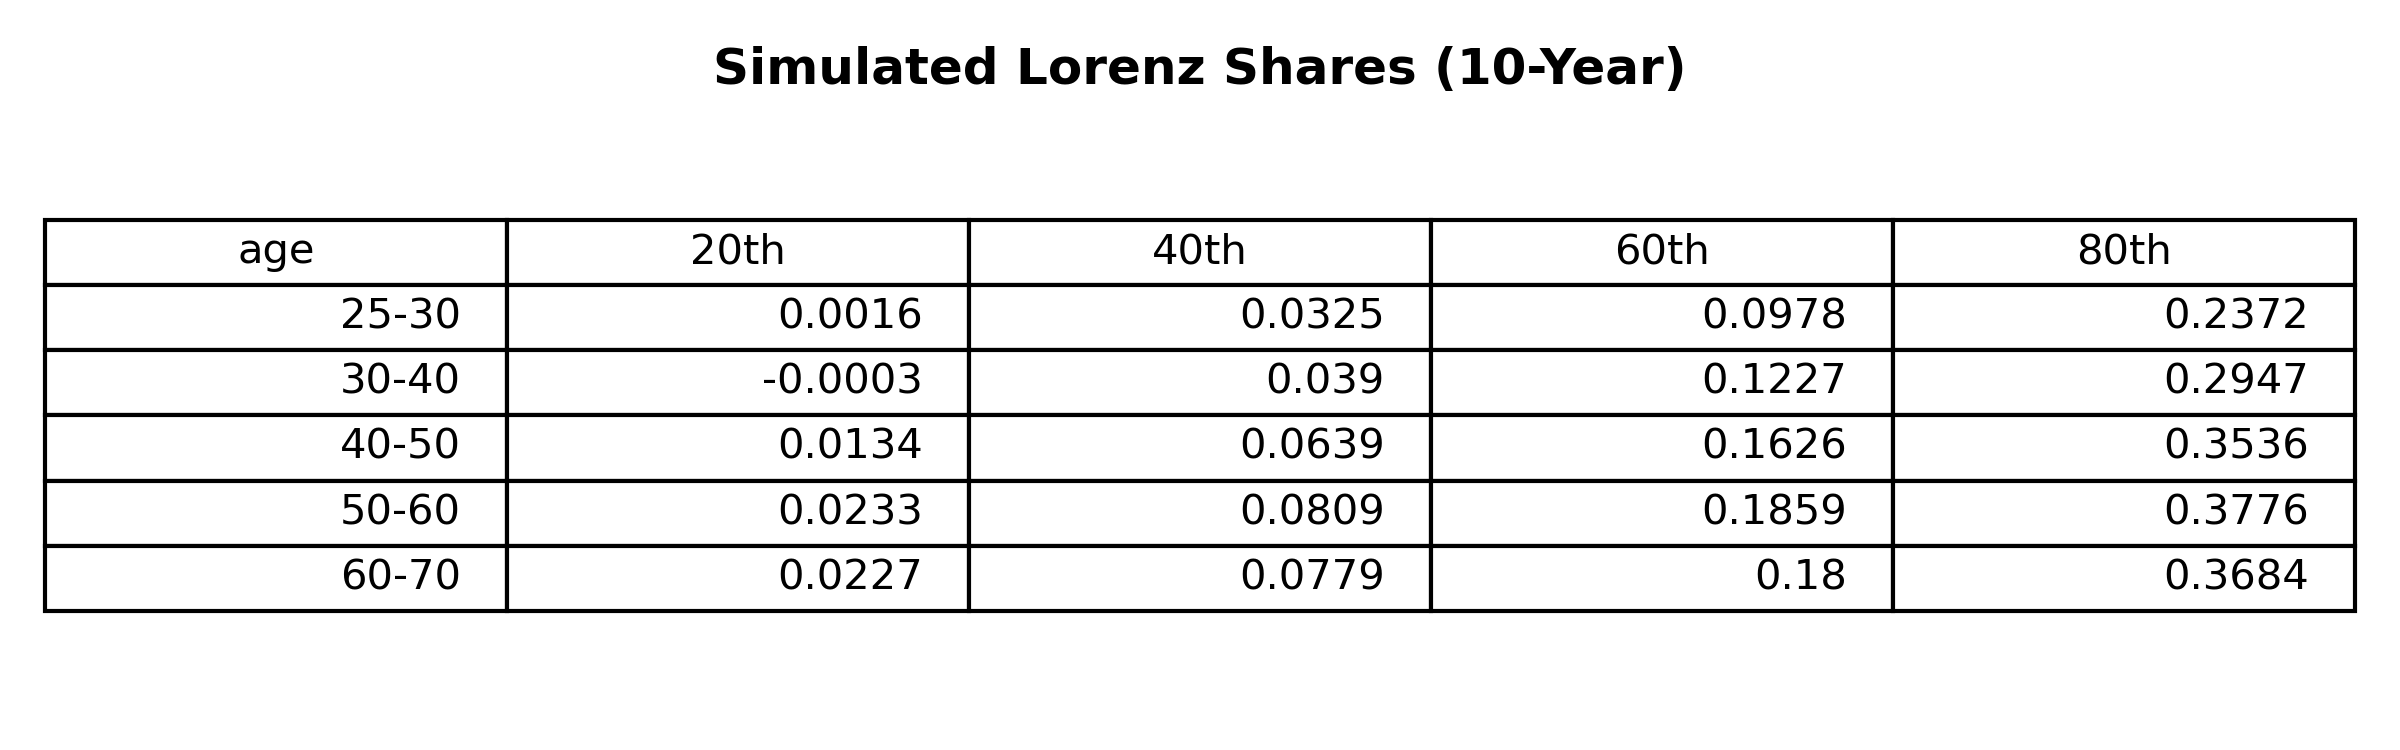
\includegraphics[width=0.8\textwidth]{Tables/Sim_Lorenz_10yr_LCrrPointNetWorth.png}
\caption{Simulated Untargeted Moments without Heterogeneity (R-point).}
\label{fig:SimLorenzTarPoint}
\end{figure}

\begin{figure}[htbp]
\centering
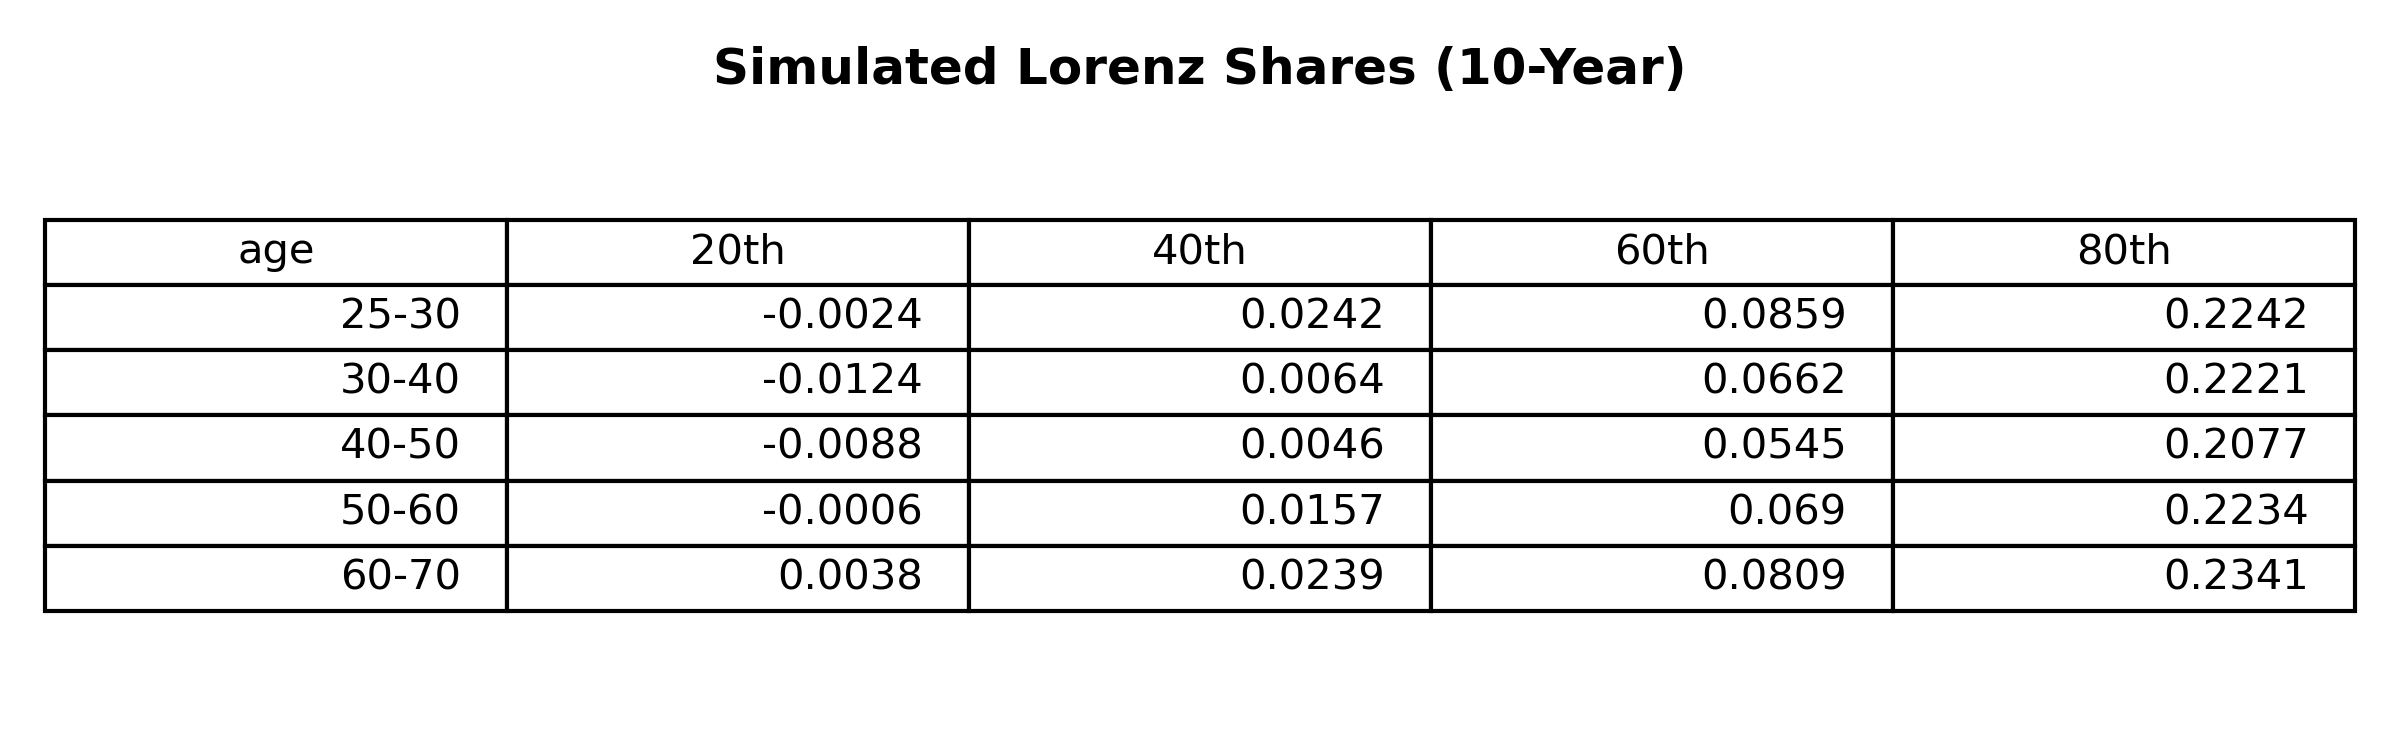
\includegraphics[width=0.8\textwidth]{Tables/Sim_Lorenz_10yr_LCrrDistNetWorth.png}
\caption{Simulated Untargeted Moments with Heterogeneity (R-dist).}
\label{fig:SimLorenzTarDist}
\end{figure}



\par 





